\documentclass[a4paper,11pt]{article}
\usepackage[left=2.5cm, right=2.5cm, top=1.5cm, bottom=1.5cm]{geometry}
\usepackage{graphicx}
\usepackage{amssymb}
\usepackage{amsmath}
\usepackage{xcolor}
\usepackage[active,tightpage]{preview}
\usepackage{hyperref}
\usepackage{pythonhighlight}

\hypersetup{ %color attributes of citation, link, etc.
    colorlinks=true,
    linkcolor=blue,
    filecolor=gray,
    urlcolor=blue,
    citecolor=blue,
}

\setlength{\parindent}{0pt}

\renewcommand{\PreviewBorder}{1in}
\newcommand{\Newpage}{\end{preview}\begin{preview}}
\newcommand{\matlab}{\textsc{Matlab}} %very important and totally necessary addition
\newcommand{\parallelsum}{\mathbin{\!/\mkern-5mu/\!}}

\newcommand\Item[1][]{%
  \ifx\relax#1\relax  \item \else \item[#1] \fi
  \abovedisplayskip=0pt\abovedisplayshortskip=0pt~\vspace*{-\baselineskip}}

%'codify' text for snippets
\usepackage{xcolor}
\definecolor{codegray}{gray}{1}
\newcommand{\code}[1]{\colorbox{codegray}{\texttt{#1}}}


\graphicspath{ {../images/} }
           
\begin{document}
\begin{preview}
\title{\LARGE{\textbf{ECEN405 Lab 5 Report\\Buck-Boost Converter}}}
\author{Niels Clayton : 300437590\\\textbf{Lab Partner:} Daniel Eisen}
\date{}
\maketitle
\hrule

\section{Design}
    $V_d=10V,\; R_L=500\Omega,\; L=4mH,\; C=100\mu F,\; D=0.6, D_{max} = 0.67$
        \subsection*{a) Switching Frequency}
            $$V_{o}=\frac{D}{1-D}V_{d}=15V$$
            $$I_{o}=\frac{V_{o}}{R_{L}}=0.03A$$
            $$I_{ripple}=0.2I_{o}\frac{V_{o}}{V_{d}}=0.009A$$
            $$I_{omax}=I_{o}+0.5I_{ripple}=0.0345A$$
            $$f_{sw}=\frac{V_{d}\left(V_{o}-V_{d}\right)}{LI_{ripple}V_{o}} = 92592Hz$$
            \begin{center}
                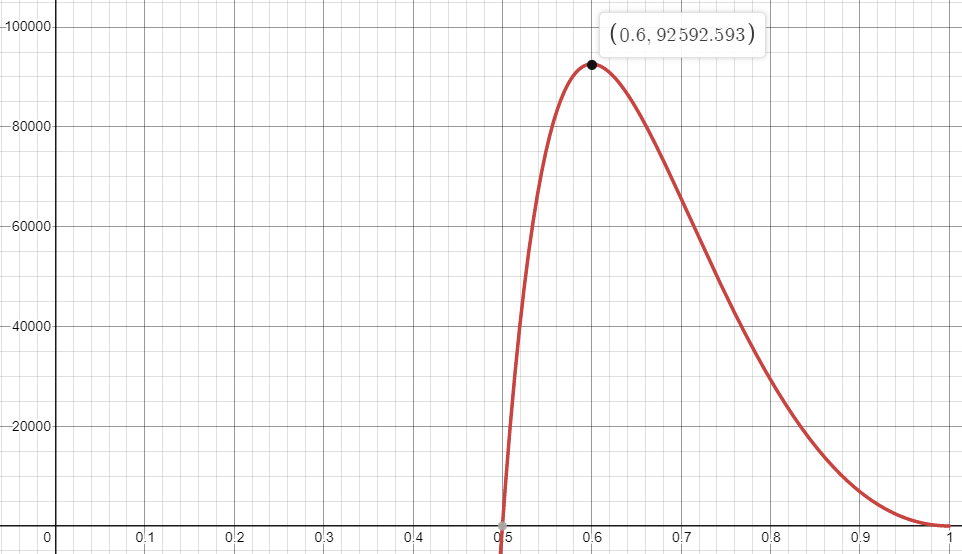
\includegraphics[width=1\textwidth]{frequency.png}\\
                \textit{Duty Cycle vs Switching Frequency}
            \end{center}
            Note that it can be seen from the plot above that a 60\% duty cycle requires the highest switching frequency. Because of this we will use this frequency rather than using the frequency for a duty cycle of 67\%, as it will guarantee a current ripple no greater than 20\% for all voltages.\\

\hrule

        \subsection*{b) Schematic}
        \begin{center}
            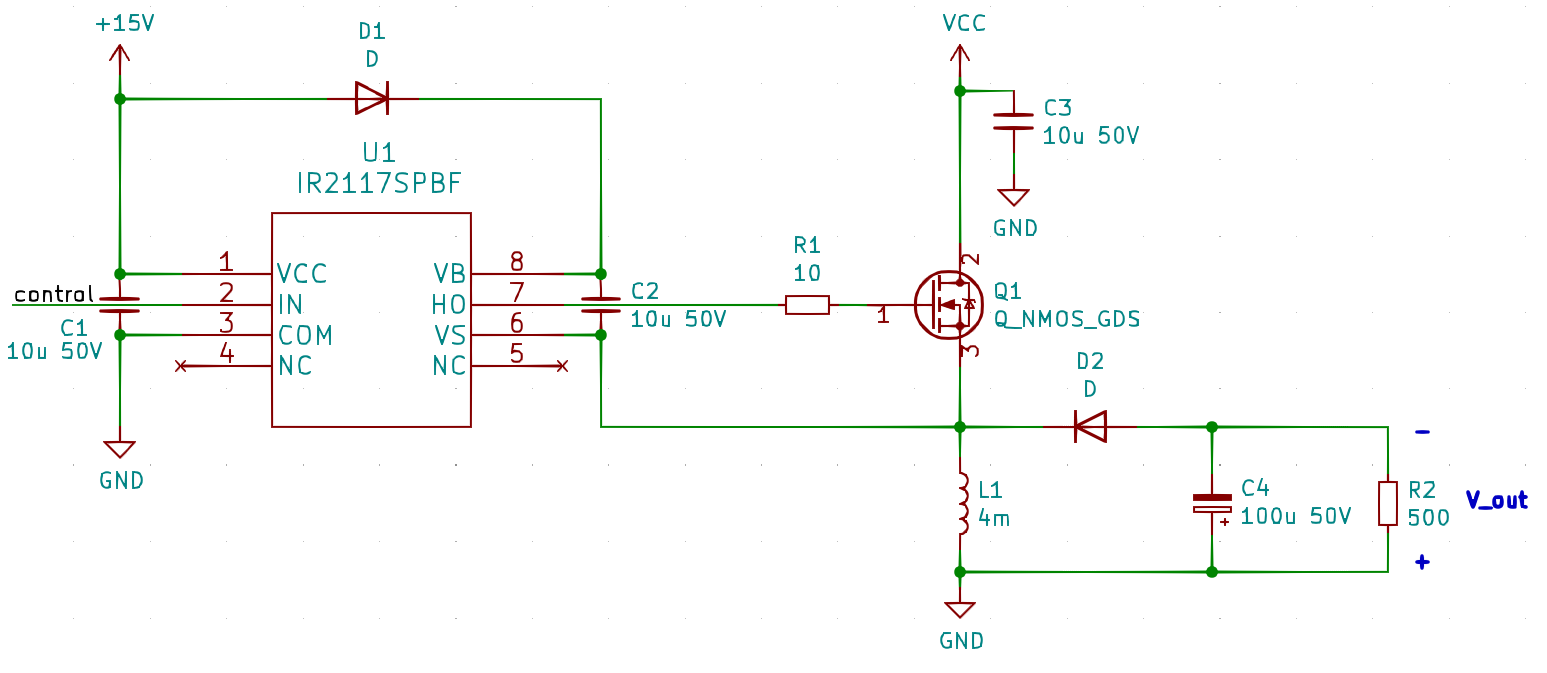
\includegraphics[width=1\textwidth]{schematic.png}
        \end{center}
        \subsection*{c) Output Voltage Ripple}
            $$V_{ripple}=\frac{I_{omax}D_{max}}{f_{sw}C}=0.00425V\\$$
      
\hrule

    \section{Output}
    The USB drive with the "real" screenshots are still in the lab plugged into the computer with a half written report on it. \\

    In light of this misplacement we have acquired an artistic recreation of the signal, based on first person accounts of the original waveform.\\

    As shown from the image below, it can be remembered that there was a substantial output voltage ripple, with possible peaks of 20 mV, and large transients at the locations of the switching.

        \begin{center}
            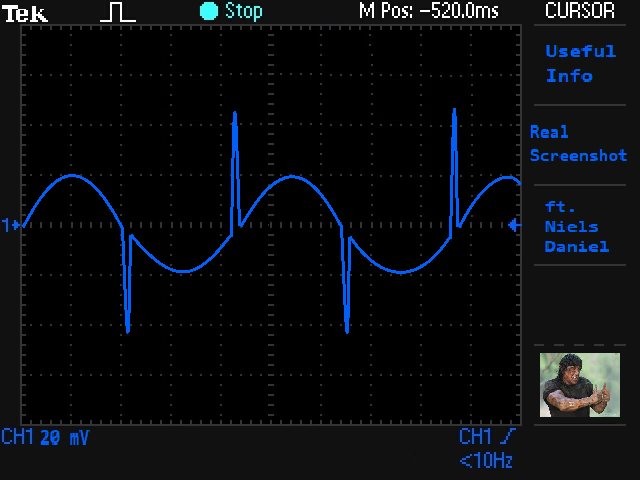
\includegraphics[width=1\textwidth]{out.png}
        \end{center}
        
\hrule

    \section{Efficiency}

    The plot below displays the efficiency vs output current plot of our designed boost converter.

        \begin{center}
            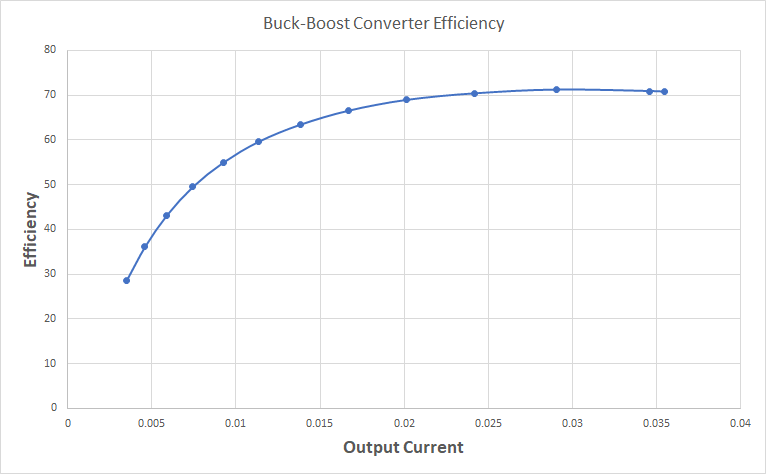
\includegraphics[width=1\textwidth]{efficiency.png}
        \end{center}


    \hrule
\end{preview}
\end{document}